\documentclass[11pt,letterpaper]{article}
\usepackage[margin=1.0in]{geometry}
\usepackage[utf8]{inputenc}
\usepackage{cite}
\usepackage{amsmath}
\usepackage{amsfonts}
\usepackage{amssymb}
\usepackage{makeidx}
\usepackage{graphicx}
\usepackage{hyperref}
\setlength\parindent{0pt}

\author{STUDENT NAME}
\title{Lab5: OpAmps and Passive Filters}

\begin{document}

\maketitle

\section{Objectives}

To understand the principle of Operational Amplifiers and their use in Amplification/Attenuation and in active low-pass and high-pass filters 

\section{Introduction}

Operational Amplifiers are low cost, simple to use and serve myriad of applications. For instance they can be used as buffers (to prevent loading errors), as amplifiers to magnify a signal’s amplitude, as well as integrator/differentiator and adders/subtractors. The latter functionality is where the Operational Amplifier gets its name.
OpAmps are near ideal amplifiers with a near infinite input impedance (up to 10 $M \Omega $), and a near zero output impedance (typically 1 $ \Omega $). The theoretical open loop amplification factor is very high, in the order of $10^6$. To obtain reasonable amplification values, external resistors are used. The resulting amplification is termed the closed loop amplification factor. When components such as capacitors are added, filters are obtained. The combination of an amplification and filter function is called an active filter. The pin layout of the 741 OpAmp is shown in Figure \ref{fig:Lab5_741OpAmp} and the complete datasheet can be found \href{http://abe-research.illinois.edu/Faculty/grift/ABE425_2015/Specs/LM741.pdf}{here}.

\begin{figure}
\centering
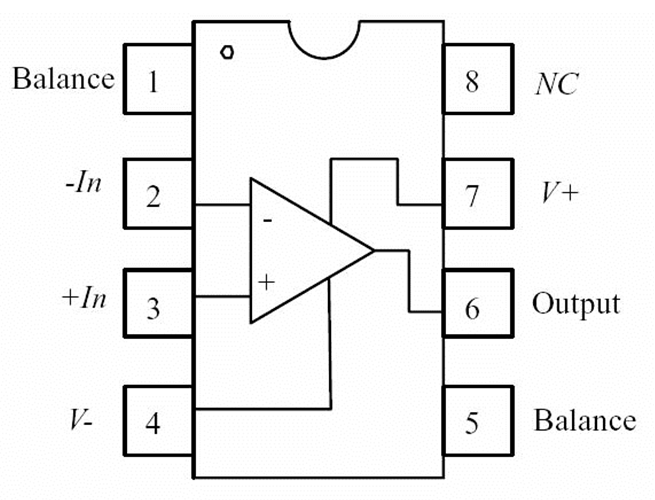
\includegraphics[width=0.6\linewidth]{Lab5_741OpAmp}
\caption{The 741 OpAmp is the most common operational amplifier on the market. The pin layout of the LM 741 Operational Amplifier is given here.}
\label{fig:Lab5_741OpAmp}
\end{figure}

\section{Equipment}

\begin{enumerate}
\item Power supply
\item Bread board
\item Resistors 10k, 100k
\item 741 OpAmp
\item Function generator
\item Oscilloscope
\end{enumerate}

\section{Procedures}

\textbf{Make a schematic all of the following assignments, and make sure the TA or instructor checks your work before you turn on the power supply.}

An OpAmp needs a positive and negative powersupply, and you need to use the DC powersupply in the lab to do that. This is potentially dangerous, make sure you know what you are doing! The two power supplies A,B are independent that means you can connect the negative terminal of supply B to the positive terminal to supply A (see Figure \ref{fig:Lab5_NegativePowerSupply}. This looks strange because in general in real life one NEVER connects a positve and negative terminal (try this on a car battery and you'll see a lot of sparks and potentially flames). However in our case we can because the supplies are independent.

\begin{figure}
\centering
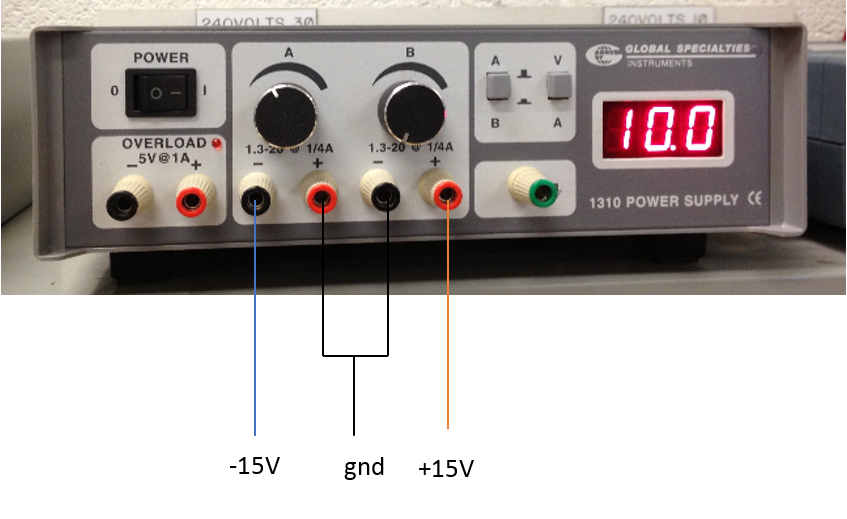
\includegraphics[width=0.8\linewidth]{Lab5_NegativePowerSupply}
\caption{To make a negative power supply, connect the negative terminal of supply B to the positive terminal of supply A. This will be your ground. Connecting a positive to a negative terminal here is allowed because the two power supplies are independent. NEVER connect the positive and negative terminals of a single powersupply!}
\label{fig:Lab5_NegativePowerSupply}
\end{figure}

\subsection{Inverting OpAmp}

The schematic of the inverting OpAmp is given in \ref{fig:Lab5_InvertingOpAmp}. The amplification formula is as follows:

\begin{figure}
\centering
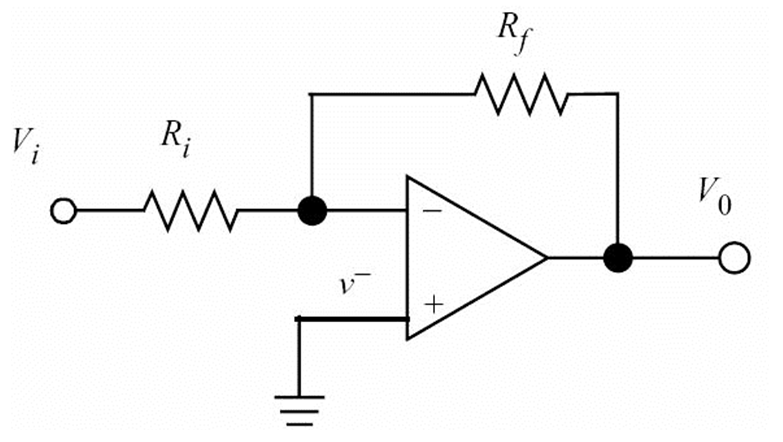
\includegraphics[width=0.6\linewidth]{Lab5_InvertingOpAmp}
\caption{Inverting OpAmp circuit.}
\label{fig:Lab5_InvertingOpAmp}
\end{figure}

\begin{equation} \label{Eqn:OpAmpsPassiveFilters1}
A = \dfrac{V_0}{V_i} = - \dfrac{R_f}{R_i}
\end{equation}

Build a circuit that amplifies an input signal of 0.5V to 5V by choosing the appropriate values of the resistors. Take some reasonably high values (for instance 10k , 100k). The power supply is + and – 15V. Do not connect the NC (Not connected) pin nor connect the balance pins. The input voltage comes from the function generator.

\begin{enumerate}
\item Measure the exact values of the resistor and compute the theoretical closed loop amplification factor
\item Apply a AC voltage with an RMS value of 0.3 Volt to the input pin. What is the amplitude of this signal? Multiply this value by the theoretical closed loop amplification factor to obtain the output voltage in RMS. Make sure to connect the ground of the power supply and the function generator for this (otherwise the input signal has no reference). Put both the input and output signals on the scope and analyze the result.
\item To determine the input resistance of the OpAmp, measure the current flowing into the device using the hand held DMM. \textbf{Be careful here: The current is measured in series, not in parallel like voltage.  Ask your TA before doing this.}
\item The amplification formula as derived is based on the assumption that there is very little voltage drop across the input terminals of the OpAmp. Measure this voltage drop and comment on how accurate this measurement is.
\end{enumerate}

\subsection{Non-inverting OpAmp}
The schematic of the non-inverting OpAmp is given in \ref{fig:Lab5_NonInvertingOpAmp}. The amplification formula is as follows:

\begin{figure}
\centering
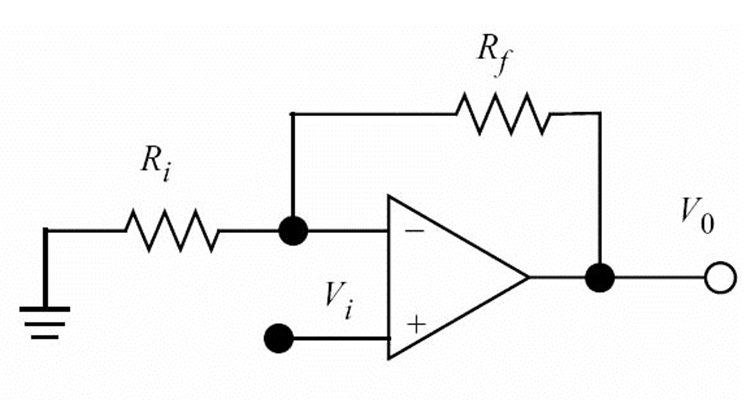
\includegraphics[width=0.6\linewidth]{Lab5_NonInvertingOpAmp}
\caption{Non-inverting OpAmp circuit.}
\label{fig:Lab5_NonInvertingOpAmp}
\end{figure}

\begin{equation} \label{Eqn:OpAmpsPassiveFilters2}
A = \dfrac{V_0}{V_i} = 1+ \dfrac{R_f}{R_i}
\end{equation}

Repeat the procedures 1,2,3 (not 4) from the inverting OpAmp section.

\subsection{Low-pass active filter}

The schematic of the low-pass active filter is given in \ref{fig:Lab5_LowPassActiveFilter}. The amplification formula is as follows:

\begin{figure}
\centering
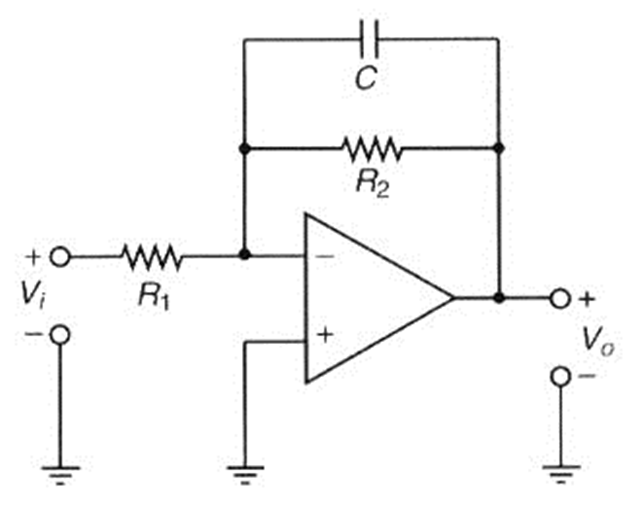
\includegraphics[width=0.6\linewidth]{Lab5_LowPassActiveFilter}
\caption{Low-pass active filter.}
\label{fig:Lab5_LowPassActiveFilter}
\end{figure}

\begin{equation} \label{Eqn:OpAmpsPassiveFilters3}
A = \dfrac{V_0}{V_i} = \left( - \dfrac{R_2}{R_1} \right)  \left(  \dfrac{1}{1 + j \omega R_2 C}  \right) 
\end{equation}

\begin{enumerate}
\item Measure the capacitor and the resistor values and compute the DC (what is the value of $\omega$ for DC?) amplification factor as well as the -3dB cutoff frequency in Hz. Generate a 0.3V pk-pk sinusoidal input signal with the cutoff frequency, and verify that the signal drops 3dB \underline{from the DC value} at the cutoff frequency. 
\item Generate a 0.3 V pk-pk square wave signal with the cutoff frequency and observe the output. Describe what you see and relate it to earlier labs.
\item Remove resistor $R_2$. What is this circuit you are left with called? Put a 0.3 V pk-pk square wave signal on the circuit and observe the output. Is this what you expected?
\end{enumerate}

\subsection{High-pass active filter}

The schematic of the high-pass active filter is given in \ref{fig:Lab5_HighPassActiveFilter}. The amplification formula is as follows:

\begin{figure}
\centering
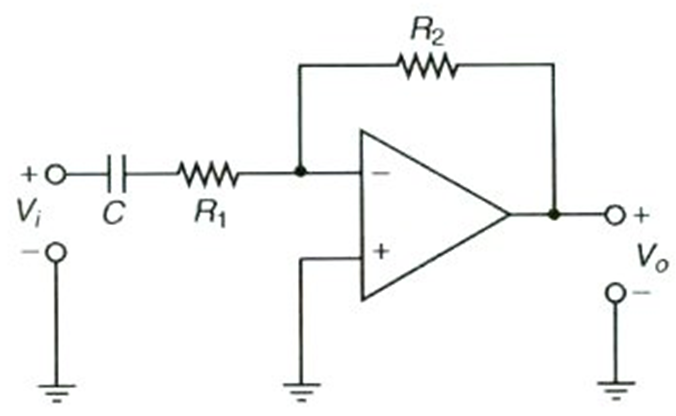
\includegraphics[width=0.6\linewidth]{Lab5_HighPassActiveFilter}
\caption{High-pass active filter.}
\label{fig:Lab5_HighPassActiveFilter}
\end{figure}

\begin{equation} \label{Eqn:OpAmpsPassiveFilters4}
A = \dfrac{V_0}{V_i} = - \left(  \dfrac{j \omega R_2 C}{1 + j \omega R_1 C}  \right) = \left( - \dfrac{R_2}{R_1}\right) \left(  \dfrac{j \omega R_1 C}{1 + j \omega R_1 C} \right)  
\end{equation}

\begin{enumerate}
\item The amplification of the high pass filter is given here. Repeat the procedures 1,2, from the low pass filter section.
\item Replace resistor $R_1$ with a wire. What is this circuit you are left with called? Put a 0.3 V pk-pk square wave signal on the circuit and observe the output. Is this what you expected?
\end{enumerate}

\section{Questions}

Q1: Explain the idea behind the Virtual Ground Principle (VGP).\\
A1:\\


Q2: Derive the transfer function of all four OpAmp circuits using the VGP. Show your results HERE using LaTex functionality.\\
A2:\\

Q3: Give the output value for a DC input for all four circuits. How does a capacitor behave for DC?\\
A3:\\


Q4: In the inverting OpAmp circuit, why is it important to choose high values for the resistors if the amplification is equal to their ratio?\\
A4:\\

Q5: Why do you have to be careful when measuring current? What is the main difference in procedure when comparing current versus voltage measurement?\\
A5:\\


Q6: 6)	If two capacitors are put in parallel, what is the resulting value? \textbf{Derive this result and show your derivation here using LaTex functionality}.\\
A6:\\


\end{document}